% Explain the implementaiton of the debug adapeter

% Overview description of the debug adapter and the flow of communication form the user to the debugger.
The debug adapter is implemanted as a \emph{TCP} server that listens for new connection on a specified port.
Then when a new connection is made it comunicates with the client using the \emph{Microsoft Debug Adapter Protocol}.
Looking at figure \ref{fig:userDAP} show the flow of comunication between the diffrent processes form the user to the debugger.
When a user interacts whith the debugger extansion in \emph{VSCode}, it will intern send a \emph{DAP} message to the debug adapter server over the \emph{TCP} connection.
The debug adapter will then process the message and translate it to commands that the debugger in the debug thread can understand and send them through a channel to the debug thread.
The debug thread will then intern procces the commands and send responsese back to the debug adapter which in tern can translate the reponse and forward it back to the \emph{VSCode} extension.
That is the normal flow of comunication but there is another case that can happen.
Which is when a event happens on the debugee, this event could be that the debugee has stoped for some reason.
In this case the flow of comunication starts at the debug thread which can be seen in figure \ref{fig:userDAP}.
The debug thread then sends the event to the debug adapter wich in tern sends it to the \emph{VSCode} extension, where it is then shown to the user by \emph{VSCode}.


% Add a flow cart of the communication? % TODO
\begin{figure}[h]
    \centering
    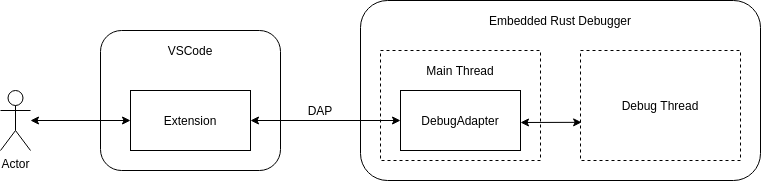
\includegraphics[width=1.0\textwidth]{user_dap_debug.png}
    \label{fig:userDAP}
\end{figure}


% Initializing the connection % TODO
It is required the the first few \emph{DAP} messages sent to the debug adapter is for configuring the debug adapter by comunicating the supported capabilities of the debugger and \emph{VSCode}.
This debugger dosen't support any of the optional capabilities that are defined in the \emph{DAP} protocol and will thus not show up in \emph{VSCode}.
After everyting is configured then the debugger will get a requires to flash the connected debugee with the program that is going to be debuged.
Now the debug adapter is started and will work as a middle man between the debugger and the \emph{GUI}.


% Explain how the debug adapter converts the DAP messages to instructions for the debugger. % TODO: remove this paragraph?
The debug adapter and the debugger is running on separate threads and thus comunicate asyncronosly using chanels.
The chanels uses a diffrent set of commands then that is defined in \emph{DAP} which means that the debug adapter translates these commands and forwards them.
This means that a single \emph{DAP} message can result in multiple commands being sent from the debug adapter to the debugger.


% Explaining how the debug adapter communicate with the debugger and wise versa. % TODO
Because the debug adapter can get messages from both the \emph{GUI} and the deugger at any time it uses continues polling on the \emph{TCP} connection and the channel.
This enables the debug adapter to forwad messages sent by both \emph{VSCode} and the debugger.

